\documentclass{scrartcl}
\usepackage[utf8]{inputenc} % Unicode support (Umlauts etc.)
\usepackage{hyperref} % Add a link to your document
\usepackage{graphicx} % Add pictures to your document
\usepackage{listings} % Source code formatting and highlighting
\usepackage[top=75px, bottom=75px, left=85px, right=85px]{geometry} % Change page borders
\usepackage{graphicx}
\usepackage{mathtools}


\begin{document}

\title{Computational Intelligence:
\\Report assignment 1}
\date{\today{}}

\author{
    \begin{tabular}{l r}
    	\\Tjitte de Jong - 4172930
	\\Boris Mulder - 4100794
        \\Max Spanoghe - 4331834
            \end{tabular}
  }
  
\maketitle \thispagestyle{empty} \pagebreak
  
\section{ANT PREPARATION: OBSERVE THE PROBLEM}
  Here we will answer the questions about the observation of the problem.
  
\subsection{}
First of all it could be possible that the ant is in a very big room. This would be difficult because it is hard to find the exit.
Secondly, it could happen that the ant gets in a dead end and needs to go back all the way.

\subsection{}
The ants drop Pheromones to let the other ants know the popularity of a certain path. The equation which determines the amount of pheromones par path is: \\
$Pheromone 
  
\begin{figure}[p]
    \centering
    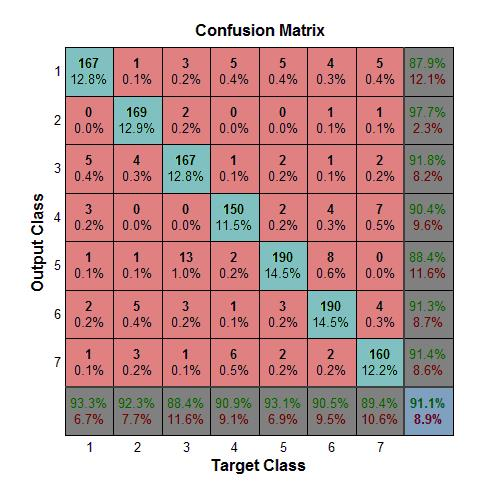
\includegraphics[width=0.8\textwidth]{Confusion_matrix.JPG}
    \caption{Confusion matrix}
    \label{fig:figure_4}
\end{figure}






 
  
\end{document}